\clearpage
\bgroup

\newcommand{\sequence}
% {seqA}  % S19 F17 S16 F16
  {seqB}  % F19 S18 S17
% {seqC}  % F18

\newcommand{\KeysseqA}
  {67,\ 23,\ 54,\ 88,\ 39,\ 75,\ 49,\  5}
\newcommand{\KeysseqB}
  {40,\ 20,\ 53,\ 85,\ 36,\ 72,\ 46,\ 17}
\newcommand{\KeysseqC}
  {53,\ 40,\ 50,\ 87,\ 37,\ 74,\ 47,\ 11}

\newcommand{\keySequenceArg}[1]{\csname Keys#1\endcsname}
\newcommand{\keySequence}{\keySequenceArg{\sequence}}

\newcommand{\qSize}
% {6} % F18
% {7} % S19 F17 S16 F16
{8} % F19 S18 S17


\Question{Hash Tables: Dealing with Collisions}

In a hash table, when two keys hash to the same location, we have a
\emph{collision}. There are multiple strategies for handling
collisions:
\begin{itemize}
\item \textbf{Separate chaining}: %
  each location in the table stores a chain (typically a linked list) of all
  keys that hashed to that location.

\item \textbf{Open addressing}: %
  each location in the table stores a key directly. In case of a collision
  when inserting, we \emph{probe} the table to search for an available storage
  location. Similarly, in case of a collision when looking up a key $k$, we
  probe to search for $k$.  Suppose our hash function is $h$, the size of the
  table is $m$, and we are attempting to insert or look up the key $k$:
  \begin{itemize}
  \item \emph{Linear probing}: %
    on the $i^\text{th}$ attempt (counting from 0), we look at index $(h(k) +
    i) \mod m$.
  \item \emph{Quadratic probing}: %
    on the $i^\text{th}$ attempt (counting from 0), we look at index $(h(k) +
    i^2) \mod m$.
  \end{itemize}
  For insertion, we are searching for an empty slot to put the key in. For
  lookup, we are trying to find the key itself.
\end{itemize}

\bigskip
\begin{parts}

\part[1]\TAGS{average-cost, complexity, hashing}
You are given a hash table of size $m$ with $n$ inserted keys.
Collisions are resolved using separate chaining. If $n = 2m$ and the
keys are \emph{not} evenly distributed, what is the worst-case runtime
complexity of searching for a specific key using big-O notation?
\begin{framed}
\bigskip
$O(\uanswer{12em}{$n$})$
\end{framed}

Under the same conditions, except that now the keys \emph{are} evenly
distributed, what is the worst-case runtime complexity of searching
for a specific key using big O notation?

\begin{framed}
\bigskip
$O(\uanswer{12em}{$1$})$
\end{framed}

As usual, for both of the answers above, give the tightest, simplest bound.

\RUBRIC
Part (a)
TAGS: average-cost, complexity, hashing

Gradescope rubric:
+ 0.5 pts O(n) --- OR --- O(m)
+ 0.5 pts O(1)

Commentary:
1/2 pt each, no partial credit
      First answer: O(n)  (or O(m))
      Second answer: O(1)
ENDRUBRIC


\newpage
\begin{EnvUplevel}
  For the next three questions, you are given a hash table of capacity
  $m = 13$. The hash function is $h(k) = k$; after hashing we attempt
  to insert the key $k$ at array index $h(k)$ mod $m$.
% We always insert at the beginning of an existing chain.
\end{EnvUplevel}

\part[1]\TAGS{hashing, testing}
Assume the table resolves collisions using separate chaining.  Show
how the set of keys below will be stored in the hash table by drawing
the \emph{final} state of each chain of the table after all of the
keys are inserted, one by one, in the order shown.
$$
\keySequence
$$
Recall that keys are inserted at the beginning of a chain.  Wherever
they occur, you should indicate \lstinline'NULL' pointers explicitly
by the notation from class: %
\raisebox{-.4\height}{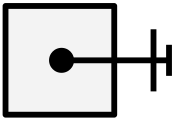
\includegraphics[scale=0.23]{\img/NULL.png}}.

\bigskip
\begin{framed}
\ifprintanswers
    \includegraphics[height=0.7\textheight]{\img/vert13-\sequence.png}
\else
  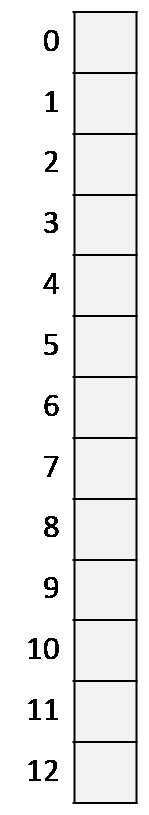
\includegraphics[height=0.7\textheight]{\img/vert13.png}
\fi
\end{framed}

\RUBRIC
Part (b)
TAGS: hashing, testing

Gradescope rubric:
+1pt EITHER --- Correct or one small error (one value in wrong chain)
+0.5pt OR --- More than 1 error but show some understanding of hash functions
-0.25pt NULL pointers not shown explicitly.

Commentary:
    1 pt if correct or one small error (one value in wrong chain but
      everything else ok),
    1/2 pt more errors but some show evidence of understanding of hash
      function

    -1/4 pt if student does not explicitly show where nulls are,
      including in array itself

    0 pts if it's a mess and shows no
      understanding of hash functions or nodes or ...

    It's fine if they write NULL instead of using the ground symbol
    They can insert entries anywhere in the chain.

   0:  NULL
   1:  53 -> 40 -> NULL
   2:  NULL
   3:  NULL
   4:  17 -> NULL
   5:  NULL
   6:  NULL
   7:  46 -> 72 -> 85 -> 20 -> NULL
   8:  NULL
   9:  NULL
   10: 36 -> NULL
   11: NULL
   12: NULL
ENDRUBRIC

% Solution for F18 sequence:
%    0:  NULL
%    1:  40 -> 53 -> NULL
%    2:  NULL
%    3:  NULL
%    4:  NULL
%    5:  NULL
%    6:  NULL
%    7:  NULL
%    8:  47 -> NULL
%    9:  74 -> 87 -> NULL
%    10: NULL
%    11: 11 -> 37 -> 50 -> NULL
%    12: NULL

% Solution for F19 sequence:
%    0:  NULL
%    1:  53 -> 40 -> NULL
%    2:  NULL
%    3:  NULL
%    4:  17 -> NULL
%    5:  NULL
%    6:  NULL
%    7:  46 -> 72 -> 85 -> 20 -> NULL
%    8:  NULL
%    9:  NULL
%    10: 36 -> NULL
%    11: NULL
%    12: NULL

% Solution for S19 sequence:
%     0:  39 -> NULL
%     1:  NULL
%     2:  67 -> 54 -> NULL
%     3:  NULL
%     4:  NULL
%     5:  5 -> NULL
%     6:  NULL
%     7:  NULL
%     8:  NULL
%     9:  NULL
%     10: 23 -> 88 -> 75 -> 49 -> NULL
%     11: NULL
%     12: NULL

\newpage
\part[1]\TAGS{hashing, testing}
Show where the keys in the sequence below are stored in the same
hash table if they are inserted one by one, in the order shown, using
\emph{linear probing} to resolve collisions.
$$
\keySequence
$$

\begin{framed}
\ifprintanswers
  \includegraphics[width=\linewidth]{\img/hor13-lin-\sequence.png}
\else
  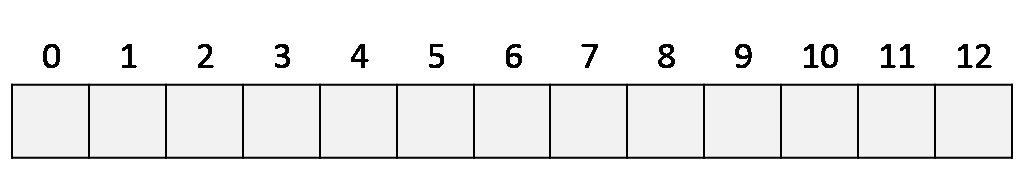
\includegraphics[width=\linewidth]{\img/hor13.png}
\fi
\end{framed}

\RUBRIC
Part (c)
TAGS: hashing, testing

Gradescope rubric:
+ 0.5 pts Some understanding of what linear probing should be doing
+ 0.5 pts Correct [39 49 67 54 -- 05 -- -- -- -- 23 88 75] or at most 1 error

Commentary:
39 49 67 54 -- 05 -- -- -- -- 23 88 75
    1 pt if correct or one small (calculation) error

    1/2 pt if more errors but shows some evidence of understanding
      of linear probing (e.g. they might put 11 in the wrong place
      since they have to wrap around... 1/2 pt)

    0 pts if wrong or shows no understanding of how linear probing works.
ENDRUBRIC
% Solution for F18 sequence:
%   11 53 40 -- -- -- -- -- 47 87 74 50 37
% Solution for S19 sequence:
%   39 49 67 54 -- 05 -- -- -- -- 23 88 75
% Solution for S17 sequence:
%   -- 40 53 -- 17 -- -- 20 85 72 36 46 --

\bigskip
\part[\half]\TAGS{hashing, testing}
Show where the keys in the sequence below are stored in the same
hash table if they are inserted one by one, in the order shown, using
\emph{quadratic probing} to resolve collisions.
$$
\keySequence
$$

\begin{framed}
\ifprintanswers
  \includegraphics[width=\linewidth]{\img/hor13-qua-\sequence.png}
\else
  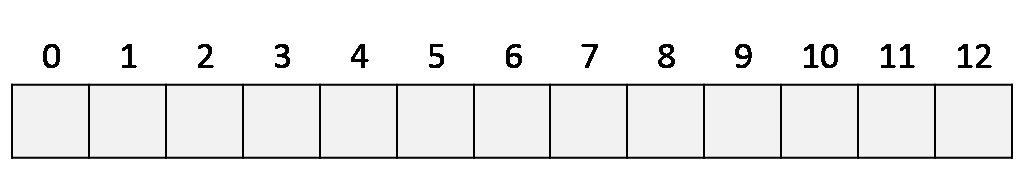
\includegraphics[width=\linewidth]{\img/hor13.png}
\fi
\end{framed}

\RUBRIC
Part (d)
TAGS: hashing, testing

Gradescope rubric:
+0.25pt First 5 inserted correctly (like linear probing)
+0.25pt Last 3 are inserted correctly

Commentary:
  39 75 67 54 -- 05 49 -- -- -- 23 88 --
    1/2 pt if correct or one small (calculation) error

    1/4 pt if the first 5 are inserted correctly (similar to linear
      probing), then goes wrong (this is where quadratic probing shows
      itself clearly)

    0 pts if wrong or shows no understanding of how any probing works.
ENDRUBRIC
% Solution for F18 sequence:
%   -- 53 40 -- -- -- -- 11 47 87 74 50 37
% Solution for S19 sequence:
%   39 75 67 54 -- 05 49 -- -- -- 23 88 --
% Solution for S17 sequence:
%   -- 40 53 46 17 -- -- 20 85 -- 36 72 --

\bigskip
\part[1]\TAGS{hashing, testing}
Quadratic probing suffers from one problem that linear probing does
not.  Given a non-full hash table, insertions with linear probing will
always succeed, while insertions with quadratic probing might not
(i.e., they may never find an open spot to insert).

Using $h(k) = k$ as your hash function and $m = \qSize$ as your table
capacity, give an example of a table with load factor not above $2/3$ and
a key that cannot be successfully inserted into the
table. (\emph{Hint:} start entering different multiples of $\qSize$.)

\medskip
\begin{framed}
\vspace*{-2ex}
\ifprintanswers
  \includegraphics[height=2.2cm]{\img/hor\qSize-sol.png}
\else
  \includegraphics[height=2.2cm]{\img/hor\qSize.png}
\fi
\vspace{0.25in}

Key that cannot successfully be inserted: \uanswer{12em}{\qSize{}0}
\end{framed}

\RUBRIC
Part (e)
TAGS: hashing, testing

Gradescope rubric:
+ 0.5 pts Enters in 4 numbers that can be entered into the hash table
+ 0.5 pts Correctly indicates a value that cannot be added

Commentary:
  Let k be the table length.  Use the case that matches k in the question.

k=6:
  The pattern of insertions from quadratic probing looks like this:
       0     1     2     3     4     5
  [ XXX | XXX |     | XXX | XXX |     ]

  So you could insert 6, 12, 18, 24 and then try to insert 60
  You could equally well insert 0, 1, 2, and 4 and then try to insert 60
  The key is that there should be four things in the table, in
   -- the place where you want to insert the uninsertable thing
   -- the place where you want to insert the uninsertable thing + 1 (mod 6)
   -- the place where you want to insert the uninsertable thing + 2 (mod 6)
   -- the place where you want to insert the uninsertable thing + 4 (mod 6)

  +1/2 pt for hashing the keys in the hint first
  +1/2 pt for hashing another value that can't go into table (a
    multiple of 6).

k=7:
  The pattern of insertions from quadratic probing looks like this:
       0     1     2     3     4     5     6
  [ XXX | XXX | XXX |     | XXX |     |     ]

  So you could insert 7, 14, 21, 28 and then try to insert 70
  You could equally well insert 0, 1, 2, and 4 and then try to insert 70
  The key is that there should be four things in the table, in
   -- the place where you want to insert the uninsertable thing
   -- the place where you want to insert the uninsertable thing + 1 (mod 7)
   -- the place where you want to insert the uninsertable thing + 2 (mod 7)
   -- the place where you want to insert the uninsertable thing + 4 (mod 7)

  +1/2 pt for hashing the keys in the hint first
  +1/2 pt for hashing another value that can't go into table (a
    multiple of 7).

k=8:
  The pattern of insertions from quadratic probing looks like this:
       0     1     2     3     4     5     6     7
  [ XXX | XXX |     |     | XXX |     |     |     ]

  So you could insert 8, 16, 24, 32 and then try to insert 80
  You could equally well insert 0, 1, 2, and 4 and then try to insert 80
  The key is that there should be three things in the table, in
   -- the place where you want to insert the uninsertable thing
   -- the place where you want to insert the uninsertable thing + 1 (mod 8)
   -- the place where you want to insert the uninsertable thing + 4 (mod 8)

  +1/2 pt for hashing the keys in the hint first
  +1/2 pt for hashing another value that can't go into table (a
    multiple of 8).
ENDRUBRIC

\end{parts}
\egroup
